%!TEX root = ../thesis.tex
%*******************************************************************************
%*********************************** First Chapter *****************************
%*******************************************************************************

\chapter{Total Monte Carlo propagation of nuclear data uncertainties to nuclear fusion engineering parameters} %Title of first chapter
\label{chap:tmc}

\ifpdf
    \graphicspath{{Chapter1/Figs/Raster/}{Chapter1/Figs/PDF/}{Chapter1/Figs/}}
\else
    \graphicspath{{Chapter1/Figs/Vector/}{Chapter1/Figs/}}
\fi

%\nomenclature[g-pi]{$\pi$}{ $\simeq 3.14\ldots$}

\section{Outline}
This chapter describes the two principal methods for uncertainty propagation used in a nuclear engineering context, the sensitivity / perturbation theory approach and a sampling method known as Total Monte Carlo. The methods and their potential applications are described. Then, examples of uncertain nuclear fusion interaction data are given, before the TMC method is applied to propagate uncertainties from fundamental nuclear physics parameters to the Tritium Breeding Ratio in a proposed nuclear fusion reactor design, DEMO. The probability distribution function of the TBR is given, along with relationships between input parameters and the TBR, and the intermediate step (cross-sections) and the TBR. Finally, comment on the relevance and consequences of the skewed TBR distribution is given in the conclusion.

%%%% OUTLINE GOES HERE

%********************************** %First Section  **************************************
\section{Introduction}
\label{introduction}
Prior to any discussion of uncertainty propagation techniques, it is worth giving some background on the problem to be studied, namely the process of producing hydrogen-3, or tritium, in a fusion device. This success of this process is crucial for the feasibility of nuclear fusion electricity, and the blanket systems which will contain the tritium producing materials and infrastructure are a significant projected fraction of any plant's capital cost. As such, reducing the uncertainty on any tritium breeding estimates is of great amenity to fusion's development as a future power source.

\FloatBarrier
\subsection{Tritium breeding}
A handful of different fusion fuels were discussed in the opening chapter. The cross-section and Q-value of the D-T reaction make a burning plasma the most easily realisable. However, sustainably liberating energy from the D-T fusion reaction requires a reliable supply of tritium fuel. Given tritium is not naturally occuring, with a $t_{\frac{1}{2}}=12.3y$ \nomenclature[a]{$t_{\frac{1}{2}}$}{Half-life} it must be artificially produced. It is worth considering whether this could be outsourced to a third party given the complexity of `grow-your-own'. The HWR reactors of Canada, Romania and the Republic of Korea produce small amounts of tritium each year, but significantly less than is required for the operation of a fusion power plant. In fact, these facilities will struggle to provide the relatively small amounts of tritium necessary for the start-up of a device \cite{Kovari2018}. Given that, future plant must be tritium self-sufficient. Neutrons will initiate tritium producing reactions in $^{6,7}$Li contained within a blanket. Depending on the blanket design, the tritium will either be purged or natually `outgas' before filtration and storage. 

The ratio of tritium produced to tritium consumed is known as the Tritium Breeding Ratio (TBR). An equation for the TBR is given as equation~\ref{eq:tbr} where $T_{prod}$ is tritons produced in the blanket, $T_{cons}$ tritons consumed in the plasma, $N_{s}$ the number density of each nuclide, $\sigma_{r}$ the r\textsuperscript{th} tritium producing reaction cross-section for that nuclide and $\phi(E)$ the neutron flux as a function of energy. 

\begin{equation}
  \label{eq:tbr}
  \mathrm{TBR} = \frac{T_{prod}}{T_{cons}} = \frac{\sum_{s=1}^{S} N_{s}}{T_{cons}} \int_{0}^{\infty} \phi(E) \sum_{r=1}^{R} \sigma_{r}(E) dE
\end{equation}

Two reactions in lithium produce the majority of tritium in the blanket and are shown below. Both naturally occuring lithium isotopes have an anomolously low nuclear binding energy per nucleon. This is why \textsuperscript{6}Li can exothermically fission despite being such a light nuclide. With the reaction being exothermic, its likelihood gains with decreasing interaction energy, meaning neutrons of all energies may potentially contribute to tritium production. Conversely, the tritium producing \textsuperscript{7}Li reaction is endothermic, with a threshold interaction energy of approximately 2.47 MeV. Natural lithium is $\approx 7.5\%$ \textsuperscript{6}Li with the remainder \textsuperscript{7}Li. Fusion breeding blankets will need their \textsuperscript{6}Li to be isotopically enriched to achieve an acceptable TBR.

\begin{equation}
\begin{split}
  ^{6}\mathrm{Li} + \mathrm{n} & \rightarrow \alpha + \mathrm{T} + 4.8\mathrm{MeV} \\
  ^{7}\mathrm{Li} + \mathrm{n} & \rightarrow \alpha + \mathrm{T} + \mathrm{n} - 2.5\mathrm{MeV}
\end{split}
\end{equation}

There are other reactions for creating tritons. For instance, the tritium decay product, $^{3}\mathrm{He}$ has an affinity for thermal neutrons and can be transmuted back to tritium by them. There is also a small chance of neutron capture leading to tritium production in $^{10}\mathrm{B}$.

\begin{equation}
\begin{split}
  ^{3}\mathrm{He} + \mathrm{n} & \rightarrow p + \mathrm{T} \\
  ^{10}\mathrm{B} + \mathrm{n} & \rightarrow 2\alpha + \mathrm{T}
\end{split}
\end{equation}

There also a variety of multi-step pathways which produce tritium via the creation of other intermediate nuclides. 

Within all proposed breeding systems there are a variety of tritium loss mechanisms: absorption in materials, leakage in the tritium extraction system and radioactive decay. To accommodate these losses and still retain a TBR in excess of unity, a margin, $M$ is employed: $\mathrm{TBR} = 1 + M$. There is a constraint on the maximum allowable tritium inventory at a given facility on the order of kilograms. The window of adequate tritium supply is therefore relatively narrow and TBR should be precisely known and/or adjustable to keep within this window. Unfortunately there are many sources of uncertainty within TBR calculations. These can broadly be categorised as: poor/missing nuclear data, modelling simplifications and Monte-Carlo statistical uncertainty. Nuclear data often contributes the greatest uncertainty to TBR \cite{El-Guebaly2009}. However, the effect of these uncertainties is rarely reported alongside calculated TBR values. This is in large part due to the difficulty of propagating uncertainty data through a Monte-Carlo radiation transport simulation to the uncertainty on integral quantities of interest. Any uncertainties that are propagated are generally based on a simplified uncertainty treatment that does not include full energy, emitted double-differential and channel-to-channel correlations. 
% ^^ needs cleaning up - does it flow in terms of concepts?

A sensitivity analysis of Helium Cooled Lithium Lead (HCLL) \nomenclature[z]{HCLL}{Helium Cooled Lithium Lead} type breeder blankets for the ITER Test Blanket Modules (TBM) \nomenclature[z]{TBM}{Test Blanket Module} has identified $^{6}$Li, $^{56}$Fe and the Pb cross-sections as the most important for TBR uncertainty \cite{Leichtle2011}. This chapter quantifies the TBR uncertainty introduced by Pb nuclear data on the HCLL DEMO blanket design by employing the Total Monte Carlo (TMC) uncertainty propagation methodology.

% \begin{figure}
% %  \figuretitle{}
%   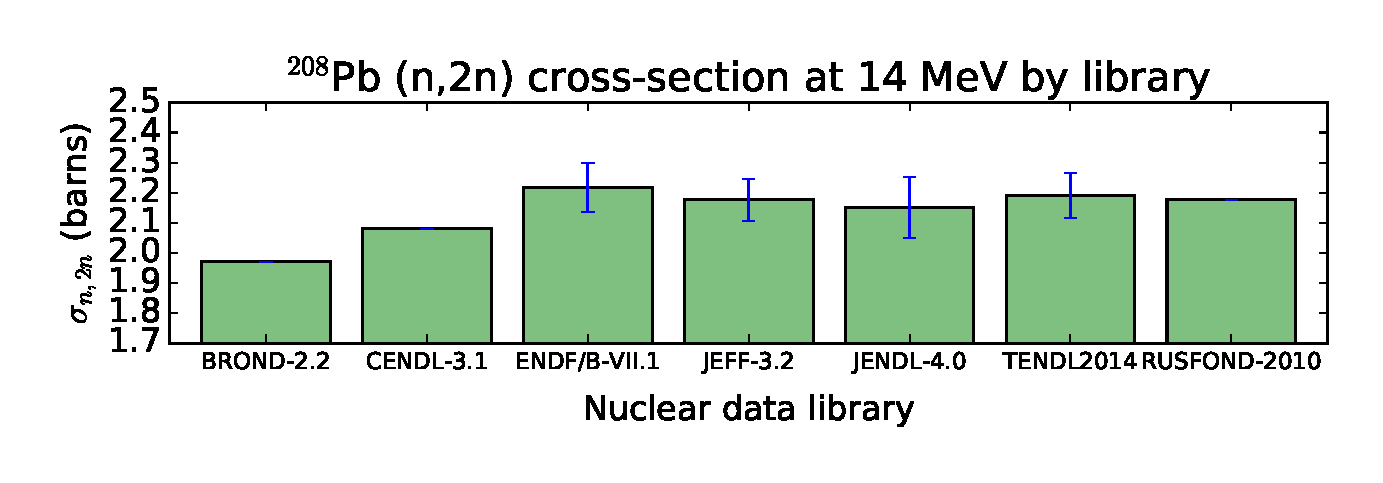
\includegraphics[width=0.47\textwidth]{pb208_n2n_by_lib}
%   \caption{$^{208}$Pb(n,2n)$^{207}$Pb cross-sections at 14MeV with their associated uncertainties for various libraries.}
%   \label{fig:lead_by_library}
% \end{figure}

% Read through section, decide on underlying topics
% Generate sub headings 
% Find papers
% Summarise and write

% HEADINGS
% Uncertainty propagation (see Michael Rising)
%   ? Conventional ?
%   Total Monte Carlo
% Uncertainty in fusion relevant nuclear data
%   Example - DT cross-section?
%   Example - Be multiplicity? O-16 scatter?
%   Example - Lead multiplicity
% END HEADINGS

\FloatBarrier
\subsection{Uncertainty propagation}
% Rising pg 90, ref 83,84
The uncertainty in ND only has intrinsic interest for ND specialists. After all, these uncertainties are a result of our lack of precision in measurement, they do not in this context arise from fundamental limits to our knowledge such as Heisenberg's uncertainty principle, for instance. Those in the nuclear engineering field who use this data are more concerned with how `integral' quantities such as heating rates, neutron fluences, TBRs, etc. are impacted by ND uncertainties. To estimate this, one must `propagate' the uncertainty from data to integral quantities. The main approaches are pertubation theory / sensitivty analysis and sampling methods. Perturbatory approaches were developed first and applied with great effect to fission reactor systems. Sampling methods only becoming available with the increases in computing power achieved in the 21\textsuperscript{st} century. The basics of the methods and the merits and demerits are described below.

\FloatBarrier
\subsubsection{Perturbation and sensitivity}
\label{subsubsec:pert}
Perturbation theory is widely applied in many branches of the sciences, and generally consists of substituting an unsoluble equation for a related, soluble one plus some perturbatory series of terms. These increasing order terms have less and less impact on the result and the series is truncated at some point. 

Work on applying this approach to reactor physics problems was undertaken by Wigner on the first nuclear pile \cite{Rising2012}. A more sophisticated framework was developed by Gandini, the Generalised Perturbation Theory (GPT) \cite{Gandini1967} and subsequently into the Equivalent Generalised Perturbation Theory (EGPT) \cite{Gandini1986}. These efforts require obtaining the forward and adjoint solutions to the Boltzmann transport equation such that one can identify the magnitude of responses to any input perturbation. This means GPT and EGPT naturally lend themselves to deterministic methods for radiation transport, where full solutions to the Boltzmann equation are obtained, rather than a subsection of its phase space sampled (as in stochastic methods). This was overcome relatively recently for fission with codes like TSUNAMI-3D by Rearden, which can calculate uncertainties in $k_{\mathrm{eff}}$ with deterministic or Monte Carlo methods \cite{Rearden2004}. An alternative method, not specific to fission problems, is to couple a radiation transport code such as MCNP \cite{goorley2012} with the SUSD or SUS-3D codes \cite{Kodeli2001}. MCNP is used with perturbed cross-sections to determine how sensitive, $S$, a response parameter, $R$, is to changes, $\delta \sigma_{g}$, in a cross-section group, $\sigma_{g}$, as shown in equation~\ref{eq:sensitivity}. 

\begin{equation}
  \label{eq:sensitivity}
  S = \frac{(\delta R)/R}{(\delta \sigma_{g}) / \sigma_{g}}
\end{equation}

SUS-3D can be used to combine processed covariance information with these sensitivity profiles to determine the uncertainty in various response parameters. Further detail on perturbation theory applied to radiation transport systems can be found in \cite{Sabouri2013}.

A disadvantage of perturbation theory methods is that they are only valid for `small' perturbiations in input quantities, which is unfortunate if some nuclear data evaluation is particularly poorly known and so of most importance to propagate. Equation~\ref{eq:sensitivity} also embodies a linear relationship between input and output uncertainty. Another disadvantage is perturbation approaches may yield the variance in some integral quantity due to a varied input, but not the higher-order moments of any distribution. Hence the skewness or kurtosis cannot be known. Even if this were possible, covariance matrices are based on normally distributed uncertainties, whether or not this is the case. Additionally, the method is very much dependent on the quality and comprehensiveness of covariance matrices available. Very large and difficult to compile covariances matrices are required to record the potential correlations between all open reaction channels. 

\nomenclature[z]{GPT}{Generalised Perturbation Theory} 
\nomenclature[z]{EGPT}{Equivalent Generalised Perturbation Theory} 
\nomenclature[z]{TSUNAMI-3D}{Tools for Sensitivty and Uncertainty Analysis Methodology Implementation in three Dimensions}

\FloatBarrier
\subsubsection{Total Monte Carlo}
\label{subsubsec:tmc}
Koning and Rochman developed a new, integrated method of uncertainty propagation in the late 2000s \cite{Koning2008}. This approach, known as Total Monte Carlo (TMC), relies on repeated sampling of varied nuclear data. Whichever problem is being investigated is simulated multiple times with different data, building a distribution of outcomes. It is a fundementally different method to the sensitivity / perturbation approach. 

The foundation is a reliable methodology for generating nuclear interaction data. The software package T6 \cite{Koning2005} collects together various frameworks for analysing nuclear interactions. Some of these are listed below:

\begin{itemize}
  \item Optical model
  \item Compound nucleus model
  \item Direct reaction model
  \item Pre-equilibrium model
  \item Fission models
  \item Nuclear structure information
  \item R-Matrix theory
\end{itemize}

Using these tools and a set of input parameters, reaction likelihoods and outcomes can be simulated for a variety of incident particles: neutron, photons, protons, deuterons, tritons helions and alpha-particles and for a range of energies from $10^{-5}\mathrm{eV}$ to $200\mathrm{MeV}$. The theoretical models require parameters which may be directly experimentally measured, or are estimated through fitting to other, robust experimental data such as total cross-sections, $\sigma_{t}$. The RIPL-3 nuclear parameter database \cite{Capote2009} contains reference values and confidence estimates for many of these parameters. These and other sources have been assimilated and parsed to provide default values for Talys, with variances. 

\begin{figure}
  \centering
  \includegraphics[width=\textwidth]{t6_flow.png}
  \caption{Nuclear data generation flowchart for the T6 software package. Figure from \cite{Koning2013}.}
  \label{fig:t6_overview}
\end{figure}

A set of nuclear parameters, $\vec{A} = [A_{1},\ldots,A_{n}]$, are used as input to T6 to generate a complete ND library, with full cross-section, resonance, angular distribution, double-differential distribution, covariance, etc. information. These data are self-consistent. An example of this behaviour is where a total cross-section is well understood, it is to be expected that a reduction in one reaction channel cross-section, say elastic scattering, would correspond with an increase in another open reaction channel. This correlation is not reproduced with simple adjustment or perturbatory approaches to uncertainty propagation. Once the ND have been generated they are processed and formatted to the ENDF standard with the Tefal component of the T6 package, permitting use by all ENDF compliant codes \cite{Koning2012}. The ND generation process is shown as figure~\ref{fig:t6_overview}.

Using the above nuclear physics parameter database and models, it is possible to repeat the nuclear data generation process to create `library of libraries', containing amongst their variance the uncertainty in the underlying nuclear physics parameters, $\vec{A}$. This data is now used as input to whichever nuclear system is to be simulated. Numerous simulations are launched, each picking a new set of input data, an evaluation from the library of libraries. Whichever reaction rates or spectral quantities can be tallied for inspection and subsequent analysis--call the quantity of interest $q$. As the number of simulations, $n$, increases, any histogram of the values of $\vec{q} = [q_{1},\ldots,q_{n}]$ will converge to a probability distribution function of the most likely value and its associated uncertainty, $\sigma_{observed}$. 

In an ideal case, this observed uncertainty would all be due to the variations in nuclear data, as in equation~\ref{eq:det_variance_sum}.

\begin{equation}
  \label{eq:det_variance_sum}
  \sigma_{observed}^{2} = \sigma_{A}^{2} 
\end{equation}

Indeed this is the case for deterministic methods. With Monte Carlo methods however, answers are inherently uncertain. Rather than solving an equation to find the exact flux and associated reaction rates at every point, the system behaviour is sampled by virtual particles (see section~\ref{subsec:monte_carlo} in chapter~\ref{chap:introduction}). Monte Carlo methods depend on the Law of Large Numbers (LLN), using a large number of simulated particles to converge on some mean behaviour. Far fewer particles populate the simulation than the real system. Short of an infinite number of `source' particles, there is always an associated uncertainty. 

Therefore, in this work the observed uncertainty, $\sigma_{observed,i}$ from a simulation $i$ is composed of two components: uncertainty from the simulation method, the standard deviation $\sigma_{stat.,i}$ and uncertainty from the nuclear data, the standard deviation being $\sigma_{A,i}$. So long as these are independent, their variances sum to give the total variance, as in equation~\ref{eq:variance_sum}.

\begin{equation}
  \label{eq:variance_sum}
  \sigma_{observed,i}^{2} = \sigma_{A,i}^{2} + \sigma_{stat.,i}^{2}
\end{equation}

Assembling a histogram of the simulated values, $\vec{q}$, approximates the underlying PDF of the quantity, $q$ of interest. We can modify equation~\ref{eq:variance_sum} from the single simulation case to extract information on the nuclear data uncertainty contained within the PDF of all simulations. The average statistical standard deviation, $\overline{\sigma}_{stat.}^{2}$, shown in equation~\ref{eq:average_stat} is simply the mean value from all $n$ simulations. Substituting this for $\sigma_{stat.,i}$ we have equation~\ref{eq:average_variance_sum}. 

\begin{equation}
  \label{eq:average_stat}
  \overline{\sigma}_{stat.}^{2} = \frac{1}{n} \sum^{n}_{i=1}\sigma^{2}_{stat.,i}
\end{equation}

\begin{equation}
  \label{eq:average_variance_sum}
  \sigma_{observed}^{2} \approx \sigma_{A}^{2} + \overline{\sigma}_{stat.}^{2}
\end{equation}

If the variance due to nuclear data, $\sigma_{A}^{2}$, is to be known, one must either enforce $\overline{\sigma}_{stat.}^{2} = 0$, or otherwise find the difference between the observed and `statistical' simulation variance. 

In terms of determining this statistical simulation uncertainty, Monte Carlo codes provide an estimate of $\sigma_{stat.,i}$. Comparing this uncertainty amongst differing values of $q$ can be achieved by normalising by $q$. The Relative Standard Deviation (RSD)\footnote{Also known as the Fractional Standard Deviation (FSD)}, $R$, is given below as equation~\ref{eq:rsd} and its functional dependence on particle count as equation~\ref{eq:rsd_m}.

\begin{equation}
  \label{eq:rsd}
  R = \frac{\sigma_{stat.}}{q}
\end{equation}

\begin{equation}
  \label{eq:rsd_m}
  R \propto \frac{1}{\sqrt{m}}
\end{equation}

Where $q$ is the reported quantity mean value and $m$ is the simulation particle population count. Keeping $R$ to an arbitrarily small value, say <0.005, allows us to ignore the $\overline{\sigma}_{stat.}^{2}$ term in equation~\ref{eq:average_variance_sum} \cite{Rochman2014a}.

If only one nuclear parameter, $A_{i}$, is varied then the nuclear data uncertainty, $\sigma_{A}$ is wholly attributable to that parameter. Similarly, if only one nuclide has its nuclear parameters and hence interaction data varied, $\sigma_{A}$ represents uncertainty on $q$ from that nuclide alone. When more parameters are varied for more nuclides, the uncertainty is an ensemble of their variation. 

\nomenclature[z]{RSD}{Relative Standard Deviation}
\nomenclature[z]{LLN}{Law of Large Numbers}

The general TMC process is diagrammatically outlined in figure~\ref{fig:tmc_overview}. Compared to other methods, this approach has a variety of benefits. One advantage of this system is that one relates uncertainty in the earliest possible parameters, say the real volume potential or imaginary surface potential of the optical model to the integral quantities of most interest to end-users such as TBR or nuclear heating in a fusion context. This allows future targeting of nuclear physics research--where are resources best allocated to reduce system uncertainties? This is the idea represented by the sensitivity feedback loop in figure~\ref{fig:tmc_overview}. Of course, this methodology does not have to only vary nuclear physics parameters, one can choose to vary parameters in the simulation model, or even methodology, to determine their contribution to uncertainty. Engineering parameters, such as component dimensions, operating temperatures, nuclide atomic densities, etc. can be varied to see how uncertainty on them effects quantities of interest.

\begin{figure}
%  \figuretitle{}
  \centering
  \includegraphics[width=0.8\textwidth]{tmc_overview.png}
  \caption{Schematic overview of the TMC process. 1) Uncertainties in fundamental nuclear parameters estimated. 2) Many sets of ND generated with T6 software, sampling from fundamental parameters. 3) Nuclear system is simulated many times with generated ND, value of observable is added to PDF, eventually converging on an observable with a mean value and characteristic distribution. Figure from \cite{Koning2008}.}
  \label{fig:tmc_overview}
\end{figure}

\FloatBarrier
\subsubsection{Comparison of methods}
Sections \ref{subsubsec:pert} and \ref{subsubsec:tmc} have discussed the methods of two uncertainty propagation schemes. It is worth noting the advantages and disadvantages of each, drawing some comparisons between them to elucidate where each method might be most appropriate.

The perturbation method, using covariance information and sensitivity profiles, has much experience associated with it. It has been used to estimate uncertainties for $k_\mathrm{eff}$ and other important parameters in fission reactor physics, with success, for several decades. As such, its results are widely accepted. Many nuclear engineers view it as the `gold standard'. By contrast, whilst the idea of repeatedly simulating a system with different inputs is not new, the integrated TMC methodology, with a sophisticated ND generation package, is novel. Published in 2008, it has seen substantially less use in industry than perturbatory approaches. The nuclear industry is often slow to adopt new technology as there can be a significant volume of work required to validate results, especially where their application is safety-critical. Studies in a variety of applications have sought to benchmark and demonstrate TMC, bringing it into wider use \cite{Koning2008}\cite{Rochman2010}\cite{Sjostrand2017}\cite{Koning2012}\cite{Alhassan2013}\cite{Alhassan2014}\cite{Rochman2011a}. 

Assuming appropriate nuclear data is already available, the slowest component of either method is radiation transport by some Monte Carlo code. Combining covariance information with sensitivity profiles, or parsing results from multiple TMC simulations to assemble a PDF of some target quantity, $q$, is of minor computational burden. If the time taken for a single simulation is $T$ time units, then TMC will take $n \times T$ where convergence on some $q$ and its $\overline{\sigma}_{observed}$ typically takes $n \geq 500$ simulations\cite{Rochman2014a}. This factor of several hundred slowdown is clearly a burden for many analyses, especially those requiring many billions of source particles such as full-core fission reactor simulations, shielding analyses or similar. In the past 3 or 4 years, progress has been made in reducing the TMC time penalty. If a single calculation requires $m$ particles for convergence, so-called `Fast TMC' uses $m/n$ particles in each of the $n$ simulations. This dedicates fewer particle histories to each change in nuclear data, exploring the $A$ parameter-space more quickly, but with a larger $\sigma_{stat.}$ for each simulation. \citeauthor{Rochman2014a} indicate that ensuring the inequality $\frac{\sigma_{stat.}}{\sigma_{observed}} \leq 0.5$ holds for each simulation, equation~\ref{eq:average_variance_sum} is still valid and the scheme still computes approximately the same uncertainties as $n$ runs each with $m$ particles. This is in contrast to traditional TMC where the rule of thumb is $\frac{\sigma_{stat.}}{\sigma_{observed}} \leq 0.05$.

The TMC and perturbation schemes do not propagate variance from or through the same set of values. Perturbatory methods, where nuclear data uncertainty is held in covariance matrices, only vary information pertaining to resonances and cross-sections. While these are very important for the uncertainty of a system, they do not represent all of the existent physics. Neglected are angular distributions of scattered and emitted particles, double differential data, $\overline{\nu}$ (average neutron yield from a fission event), fission neutron energy spectra, etc. These types of data are especially important for higher energy nuclear systems such as fusion, where angular distributions are less isotropic. As TMC calculates and varies a full complement of nuclear data with its set of nuclear models, it can claim to have a more comprehensive estimate of the true uncertainty. While perturbations to generate sensitivity profiles are for a single cross-section group value (for example), TMC varies parameters at an earlier step, as a fundamental parameter for the behaviour of the nucleus. Because of this, when a parameter is varied in the TMC approach, it in turns varies all correlated phenomena. Other areas where the TMC scheme embodies a more complex approach are the assumed linearity of the perturbation method, along with the inability of perturbation methods to accommodate non-Gaussian observable distributions. Despite these advantages, the TMC method has attracted certain criticisms. It can be argued that the all-important nuclear parameter distributions have not been rigorously estimated from experimental data \cite{Helgesson2017}. Both \citeauthor{Capote2010} and \citeauthor{Rising2012} note the arbitariness of some parameter distributions. Recently, work has been undertaken to implement Bayes' theorem through the assignment of weights to generated ND \cite{Koning2015a}, based on experimental data and automatically generated covariance files \cite{Helgesson2017}.

The ease of application of the two methods is varied. While TMC is conceptually easy to understand and incorporates many advantageous features, there are limitations in its application, principally the failure of theoretical models to correctly predict the behaviour of light nuclides (the typical cut-off being fluorine) \cite{Rochman2011}. For perturbation methods, the paucity of covariance information is a problem for some calculations (principally those outside the thermal fission realm). 

\FloatBarrier
\subsection{Uncertainty in fusion relevant data}
There are many nuclides of importance in nuclear fusion studies whose behaviour are poorly known \cite{Forrest2011}. Nuclear technology development programmes for ITER \cite{Batistoni2008} and DEMO \cite{Abdou2015} have both identified the need for more widespread uncertainty estimates and more accurate nuclear data evaluations to reduce uncertainties. \citeauthor{Batistoni2008} cites conservative uncertainties for neutron fluence at the ITER pressure vessel ($\pm 15\%$) and superconducting Toroidal Field (TF) coil magnets ($\pm 30\%$) due to nuclear data uncertainties. 

An improved uncertainty treatment has been advocated for tritium breeding since the early days of detailed reactor design \cite{Abdou1986}. \citeauthor{Youssef1986} performed a sensitivity / perturbation analysis on uncertainties in TBR due to ND for early blanket designs finding that ND contributed an uncertainty on TBR of between 2--6\% of the mean value depending on the specific design. A variety of different tritium breeding schemes are proposed for reactors. These have either solid (ceramic pebbles) or liquid (molten metal) breeding compounds which may or may not be accompanied by an additional multiplying material. The solid systems have some sort of additional coolant loop, typically employing He or H\textsubscript{2}O. For the liquid metal systems, the breeder also functions as the primary coolant. All systems are likely to have a secondary coolant loop for subsequent electricity generation. \citeauthor{Youssef1986} compared the TBR uncertainty due to ND for several of these systems. He found that Li\textsubscript{2}O ceramic systems typically have a large uncertainty contribution from \textsuperscript{16}O, followed by \textsuperscript{56}Fe and the lithium isotopes (their relative importance depending on the enrichment). Uncertainty in a LiAlO\textsubscript{2} system on the other hand was dominated by uncertainty in \textsuperscript{9}Be multiplicity cross-section data. For a Li-Pb, liquid metal system, the TBR uncertainty was dominated by variance in the lead multiplicity cross-sections, the (n,2n) and to a lesser extent (n,3n) reactions.

As well as pure computation, work is available comparing simulation and experimentally determined values for important reaction reaction channels in HCPB tritium breeding systems \cite{Batistoni2007}. To my knowledge, less work has been undertaken to experimentally corroborate simulated nuclear responses in liquid metal blankets. This is not for lack of desire, these lithium-lead blankets are currently in development in tandem with the solid breeders and account for half of the Test Blanket Modules (TBM) to be tested in ITER \cite{Chuyanov2010}. There are good reasons to expect lithium-lead blankets to be further developed, including the greater resource availability (beryllium for ceramic blankets is in limited supply \cite{Bradshaw2011} \cite{Shimwell2014}), the facility for on-load lithium enrichment and thus TBR adjustment \cite{Ihli2008}, higher natural breeding ability \cite{Colling2012} and the comparative ease of extracting bred tritium from a liquid metal vs. porous pebbles. A more thorough discussion on the advantages and disadvantages of the different technologies can be found in \cite{Abdou2015}. 

%\nomenclature[z]{HCPB}{Helium Cooled Pebble Bed}
%\nomenclature[z]{HCLL}{Helium Cooled Lithium Lead}
\nomenclature[z]{TBM}{Test Blanket Module}
\nomenclature[z]{TF}{Toroidal Field}

% The other examples seem strange to include if there's not going to be any TMC analysis...
%\subsubsection{Deuterium-Tritium}
%\subsubsection{\textsuperscript{16}O scattering}
%\subsubsection{Lead multiplicity}

As briefly mentioned previously, \citeauthor{Leichtle2011} has undertaken a recent study where nuclear data was adjusted to obtain the sensitivity of TBR in a modern HCLL system (the ITER HCLL TBM) to various nuclear reaction cross-sections \cite{Leichtle2011}. This work identified $^{6}$Li, $^{56}$Fe and the Pb cross-sections as the most important for TBR uncertainty from the a ND perspective. The analysis below looks at variation in lead nuclear data. 

Cross-section uncertainties can be represented as single values for a given energy and reaction channel. As an example, the $^{208}$Pb(n,2n)$^{207}$Pb reaction at 14MeV is shown in Table \ref{tab:lead_by_lib} for a variety of nuclear data libraries. Information on how uncertainty for a given energy affects other energies is quantified in energy covariance matrices, but these are not available for the majority of reaction channels in standard nuclear data libraries.

\begin{table}[ht]
  \footnotesize
  \centering
  \begin{tabularx}{\textwidth}{XXXX}
    \toprule
    Source & Energy [MeV] & $\sigma_{n,2n}$ [b] & $\pm\%\Delta\sigma_{n,2n}$ \\
    \midrule
    BROND 2.2 & 14.0 & 1.97 & - \\
    CENDL 3.1 & 14.0 & 2.08 & - \\
    ENDF/B-VII.1 & 14.0 & 2.22 & 8.15 \\
    JEFF 3.2 & 14.0 & 2.18 & 7.0 \\
    JENDL 4.0 & 14.0 & 2.15 & 10.1 \\
    TENDL 2015 & 14.0 & 2.19 & 7.4 \\
    RUSFOND 2010 & 14.0 & 2.18 & - \\
    EXFOR: Simakov & 14.1 & 2.38 & 5.88 \\
    EXFOR: J. Frehaut & 14.28 & 1.97 & 8.57 \\
    \bottomrule
  \end{tabularx}
  \caption{Cross-section values for the n,2n reaction channel, $\sigma_{n,2n}$ around 14 MeV for various libraries and experiments. The ENDF utility code Inter \cite{Dunford2002} was used to extract the values for each library. The two experimental results were retreived from the online EXFOR database \cite{exfor2017}. The uncertainties, $\Delta\sigma_{n,2n}$ are presented as percentages above and below the reported value.}
  \label{tab:lead_by_lib}
\end{table}

\FloatBarrier
%\subsection{DEMO}
% Should this be here? Perhaps it doesn't need a whole bit...

\FloatBarrier
\section{Method}

\subsection{Nuclear data}
\label{sec:data}
This study used the TENDL-2015 library. It is a comprehensive, general-purpose nuclear data library which contains data on interactions between 7 projectiles and over 2,800 target nuclides. As described above, the library is produced by a suite of codes known as T6 and an adherance to a strict methodology of reproducability \cite{Rochman2016}. It uses the TALYS nuclear reaction code to model high-energy reactions, with TARES handling the lower energy, resonant region. The inputs are fundamental parameters, including data from the RIPL-3 database \cite{Capote2009}, each with their own probability distributions that reflect their uncertainties. The TENDL-2015 release contains `average' or best-guess evaluations, but also a collection of `random' files, those generated using the sampling method. These have been pre-generated by the TENDL team. Information on the input parameters and plots of the ND are available online \cite{TENDL2015}.

It is instructive to inspect the nuclear data used as input for this TMC simulation. The sampled nuclear data files were downloaded in both ACE (293K) and ENDF format from the TENDL-2015 website \cite{TENDL2015}. Figure \ref{fig:tendl_lead} shows the (n,2n) cross-sections as a function of energy for $^{208}$Pb. 

% \begin{figure}
% %  \figuretitle{}
%   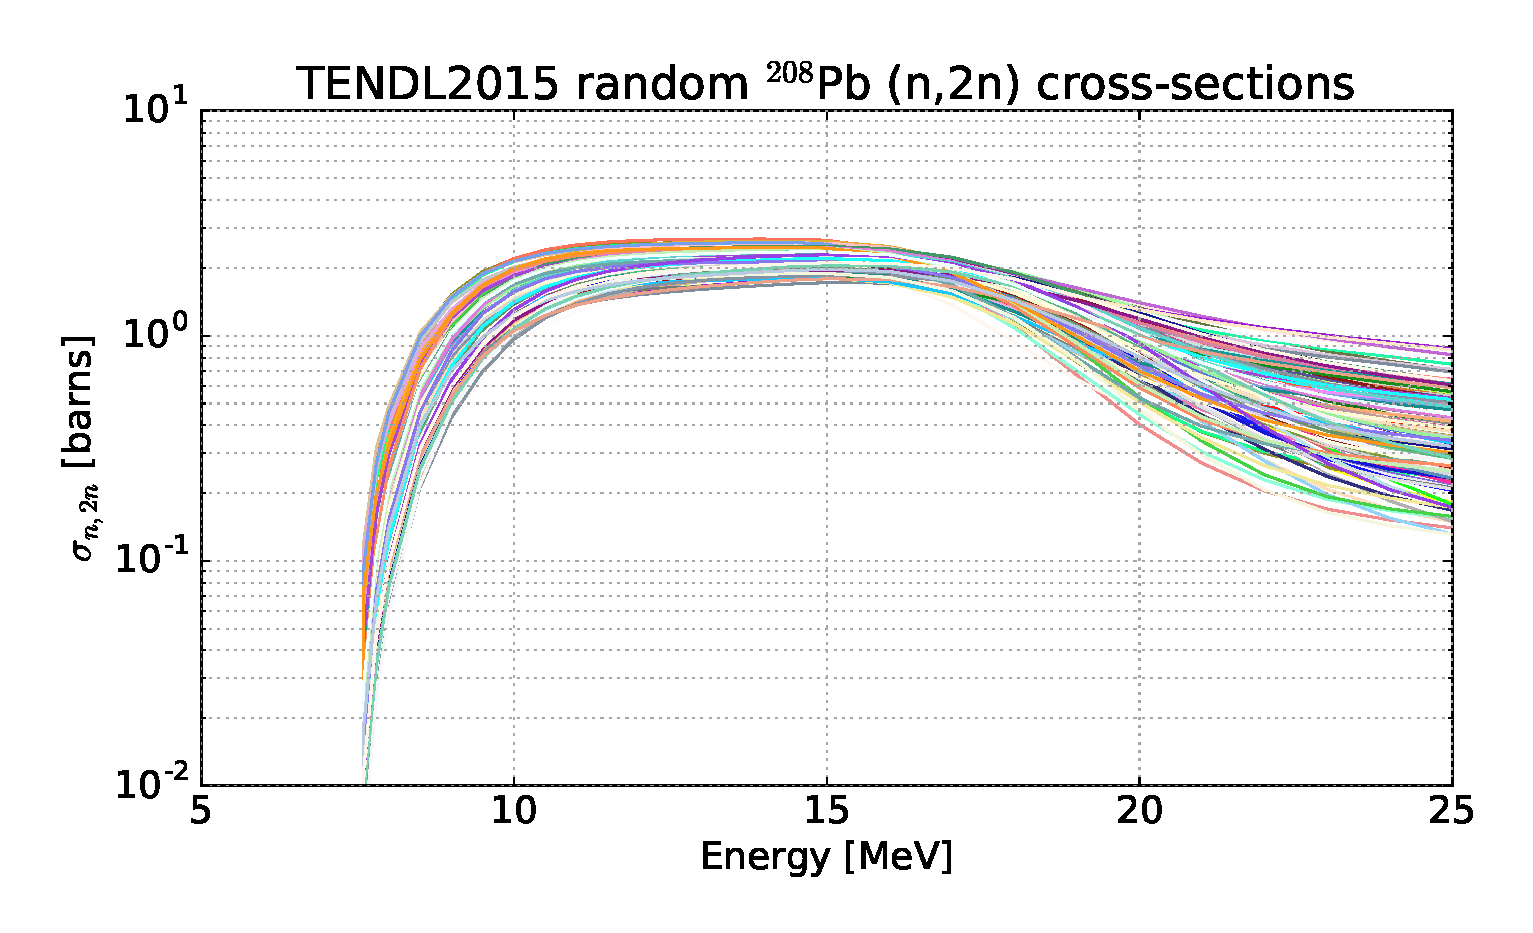
\includegraphics[width=0.48\textwidth]{pb208_tendl_n2n}
%   \caption{Shown here are 300 `random' TENDL2015 n,2n cross-sections as a function of energy for the most abundant lead isotope, $^{208}$Pb.}
%   \label{fig:tendl_lead}
% \end{figure}

\begin{figure}
%  \figuretitle{}
  \centering
  \includegraphics[width=\textwidth]{pb208_n2n_tendl_exfor.png}
  \caption{Shown here are $^{208}$Pb (n,2n) cross-sections as a function of energy. The plot shows the TENDL `random' data extracted from ACE files. Additionally, the few available experimental results in EXFOR are plotted for comparison.}
  \label{fig:tendl_lead}
\end{figure}

In an unmoderated fusion neutron spectrum the dominant reaction channels for Pb are neutron multiplication (n,2n) and elastic scattering, at approximately 2 and 3 barns respectively. The ENDF utility code Inter was used to extract cross-section values at a given energy from the ENDF files. The resulting distributions and correlations were plotted as figures \ref{fig:tendl_n2n}, \ref{fig:tendl_nel} \& \ref{fig:pb_el_n2n_corr}. Figures \ref{fig:tendl_n2n} and \ref{fig:tendl_nel} were examined for their first 3 statistical moments. 

\begin{table}[ht]
  \footnotesize
  \centering 
  \begin{tabular}{llll}
    \toprule
    Nuclide & Mean, $\mu$ [b] & RSD, $\frac{\sigma}{\mu}$ & Skewness \\
    \midrule
    Pb206 & 2.11 & 8.1\% & -0.065 \\
    Pb207 & 2.12 & 10.7\% & -0.868 \\
    Pb208 & 2.17 & 9.7\% & -0.120 \\
    \bottomrule
  \end{tabular}
  \caption{TENDL2015 `random' Pb n,2n neutron multiplicity channel cross-section distribution statistics}
  \label{table:n2n} % is used to refer this table in the text
\end{table}

Figure \ref{fig:tendl_n2n} and Table \ref{table:n2n} show the distributions of TENDL-2015 cross-sections for (n,2n) at 14MeV. Lower values for $\sigma_{n,2n}$ will reduce the neutron multiplication of the blanket and, other quantities being equal, result in a reduced total neutron flux and therefore a lower TBR.

\begin{figure}[ht]
%  \figuretitle{}
	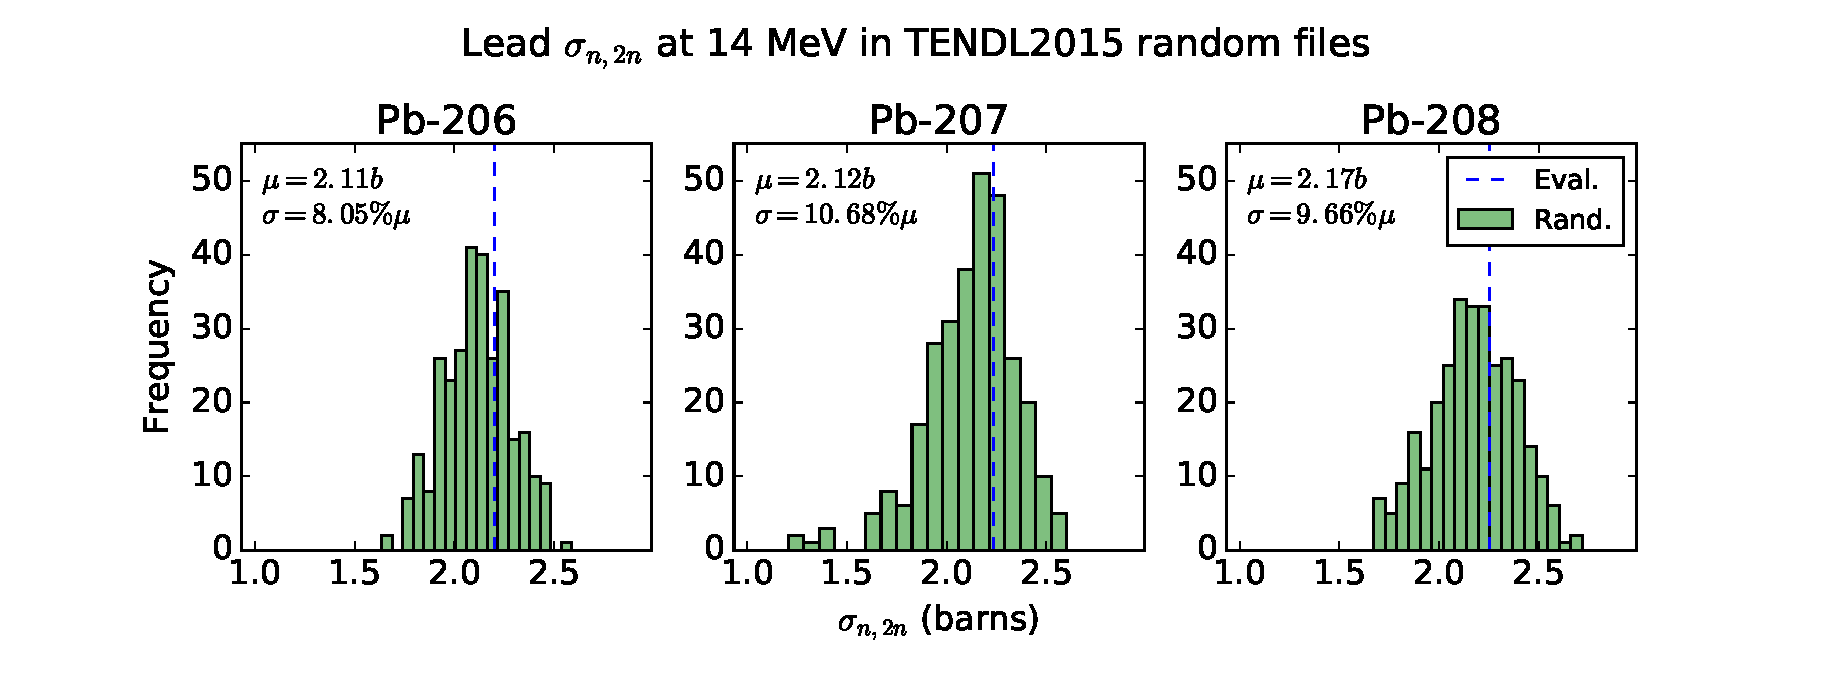
\includegraphics[width=\textwidth]{pb_tendl_n2n_hist}
	\caption{Shown are histograms of $\sigma_{n,2n}$ at 14MeV for the three major Pb isotopes. It can be seen that while $^{206,208}$Pb are approximately symmetrical with skewness values close to zero, $^{207}$Pb has a skewness of -0.868 indicating a low-value tail. This may or may not be representative of the underlying distribution. The histogram contains all 300 available files for $^{207}$Pb, but it could be the case that with more files a Gaussian shape would be recovered.}
	\label{fig:tendl_n2n}
\end{figure}

\begin{table}[ht]
  \footnotesize
  \centering 
  \begin{tabular}{llll}
    \toprule
    Nuclide & Mean, $\mu$ [b] & RSD, $\frac{\sigma}{\mu}$ & Skewness \\
    \midrule
    Pb206 & 2.84 & 7.5\% & 0.663 \\
    Pb207 & 2.80 & 8.0\% & 0.548 \\
    Pb208 & 2.81 & 8.1\% & 1.185 \\
    \bottomrule
  \end{tabular}
  \caption{TENDL2015 `random' Pb elastic scattering cross-section distribution statistics}
  \label{table:nel}
\end{table}

\begin{figure}[ht]
%  \figuretitle{}
  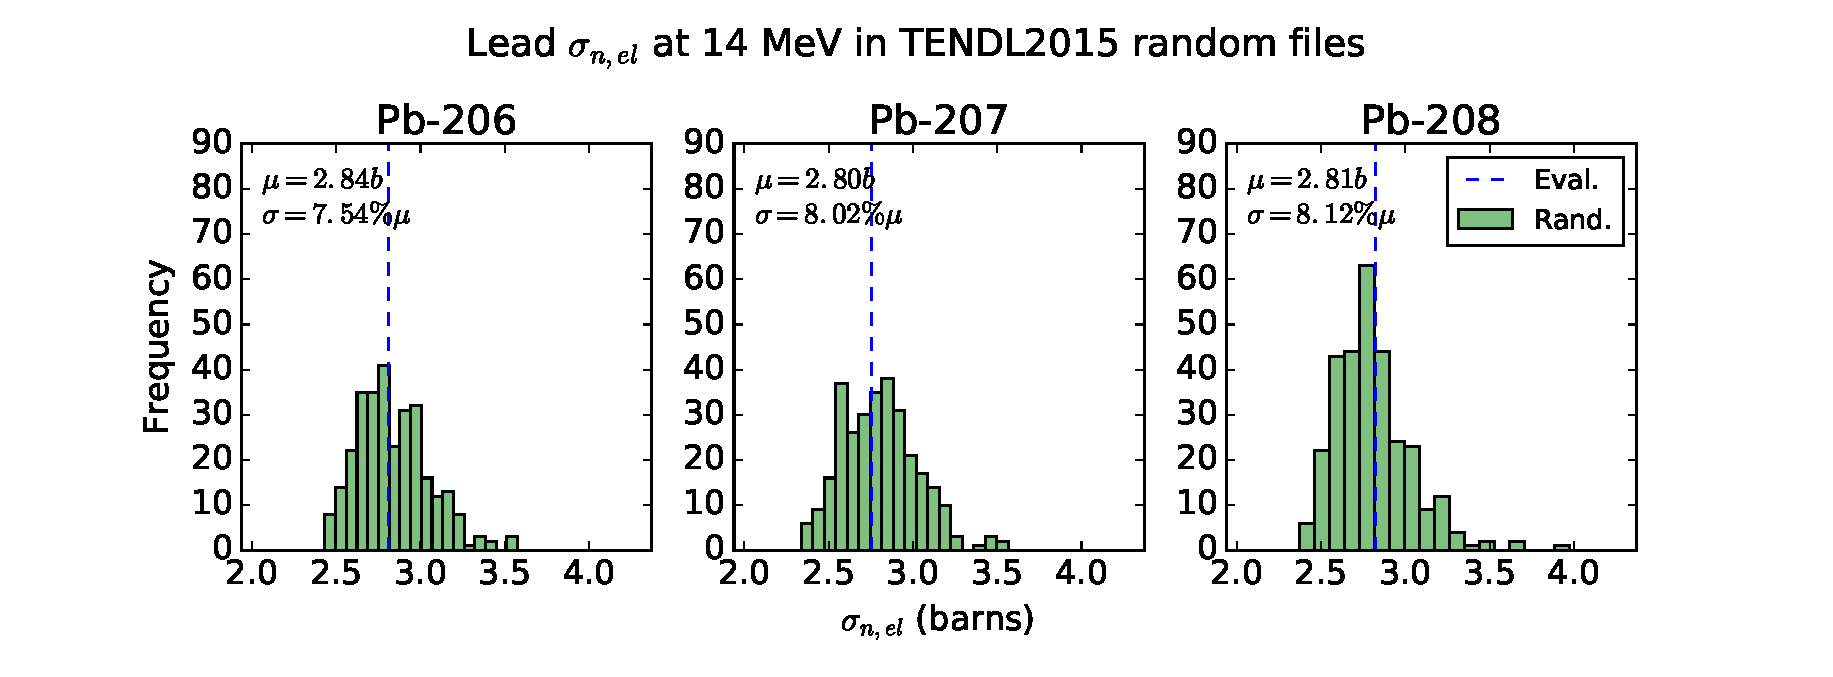
\includegraphics[width=\textwidth]{pb_tendl_nel_hist}
  \caption{The elastic scattering cross-sections for lead at 14MeV are all positively skewed, with $^{208}$Pb having a skewness value of 1.185.}
  \label{fig:tendl_nel}
\end{figure}

The elastic scattering data shown in Figure \ref{fig:tendl_nel} and Table \ref{table:nel} are instead positively skewed, with high value tails for each isotope, with the most pronounced tail being $^{208}$Pb. A greater elastic scattering cross-section will result in an increased likelihood of downscattering neutrons to lower energies. The softer spectrum will increase triton production in $^{6}$Li as the cross-section increases with decreasing energy, i.e. $\sigma_{n,t}(E) \propto \frac{1}{E}$. However, the elastic scattering cross-section is anti-correlated with the n,2n cross-section in the TENDL data (see figure \ref{fig:pb_el_n2n_corr}). In other words, a high scatter cross-section is typically coupled with a low multiplicity cross-section. This compensating effect decreases the overall uncertainty where individual perturbations on a single channel would result in an unrealistic, larger uncertainty. This inclusion of cross-channel correlation is one of the key advantages of TMC over more traditional uncertainty propagation (UP) methods. 

\begin{figure}[ht]
%  \figuretitle{}
	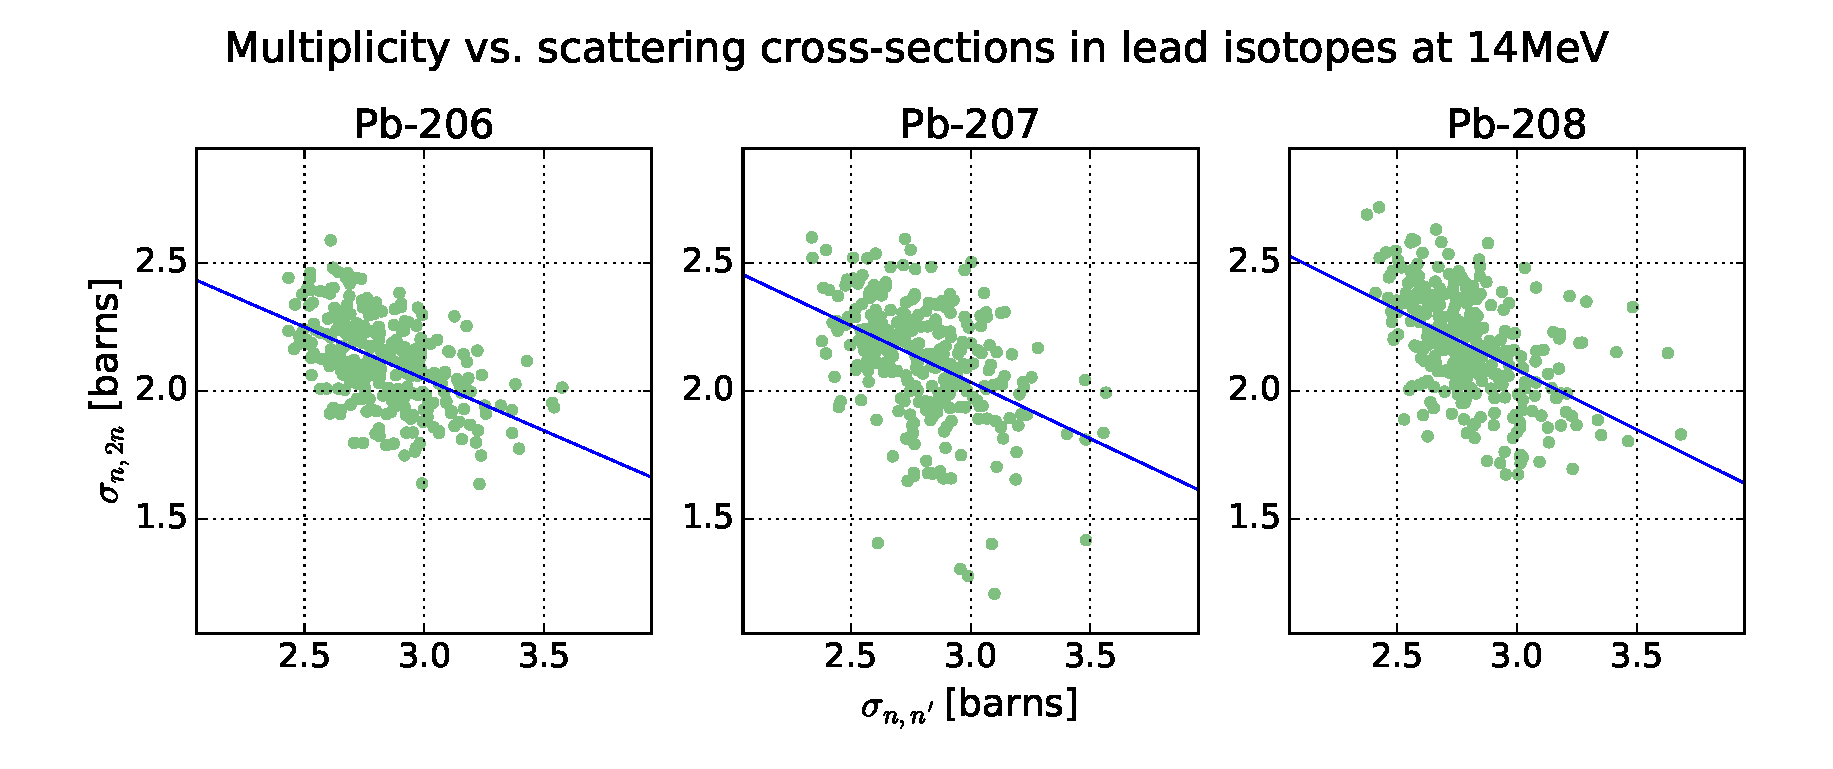
\includegraphics[width=\textwidth]{pb_el_n2n_corr}
  \caption{Shown here are scatter plots of the relationship between the scattering and n,2n cross-sections in the TENDL data. The two channels are clearly anti-correlated. A least squares fit has been applied and the resulting linear relationship plotted.}
	\label{fig:pb_el_n2n_corr}
\end{figure}

\FloatBarrier
\subsection{Radiation transport}
An 11.25\degree \ 2014 DEMO HCLL MCNP model was modified to tally TBR. The particle count was set to $3\cdot10^{6}$ giving a TBR relative standard deviation, RSD $\approx 0.002$ for each simulation. This is negligible compared to the total (nuclear data \& statistics) accumulated RSD and so the variance of the observable is assumed to be entirely due to variance in the nuclear data. While other TMC analyses have separated out the Monte-Carlo statistical variations to limit the computational cost \cite{Rochman2014a}, in this work the statistical variation has been strictly limited to avoid this issue. Whilst the Pb nuclear data employed was from TENDL-2015, FENDL3.1b data was used for the neutron transport of other elements present in the reactor model. A series of simple Bash and Python scripts were used to select different Pb TENDL-2015 ACE files for different runs, before creating and submitting jobs to the local cluster.

\section{Results \& discussion}
Python scripts were used to plot TBR convergence as a function of simulation count (see figure \ref{fig:convergence}) and the distributions of simulated TBR (see figure \ref{fig:tbr_distribution}).

The TMC simulation was run for a total of 1559 MCNP simulations, each 84 core-minutes across 32 cores. The total wall-clock time was 3 days, 15 hours.

\begin{figure}[ht]
%  \figuretitle{}
	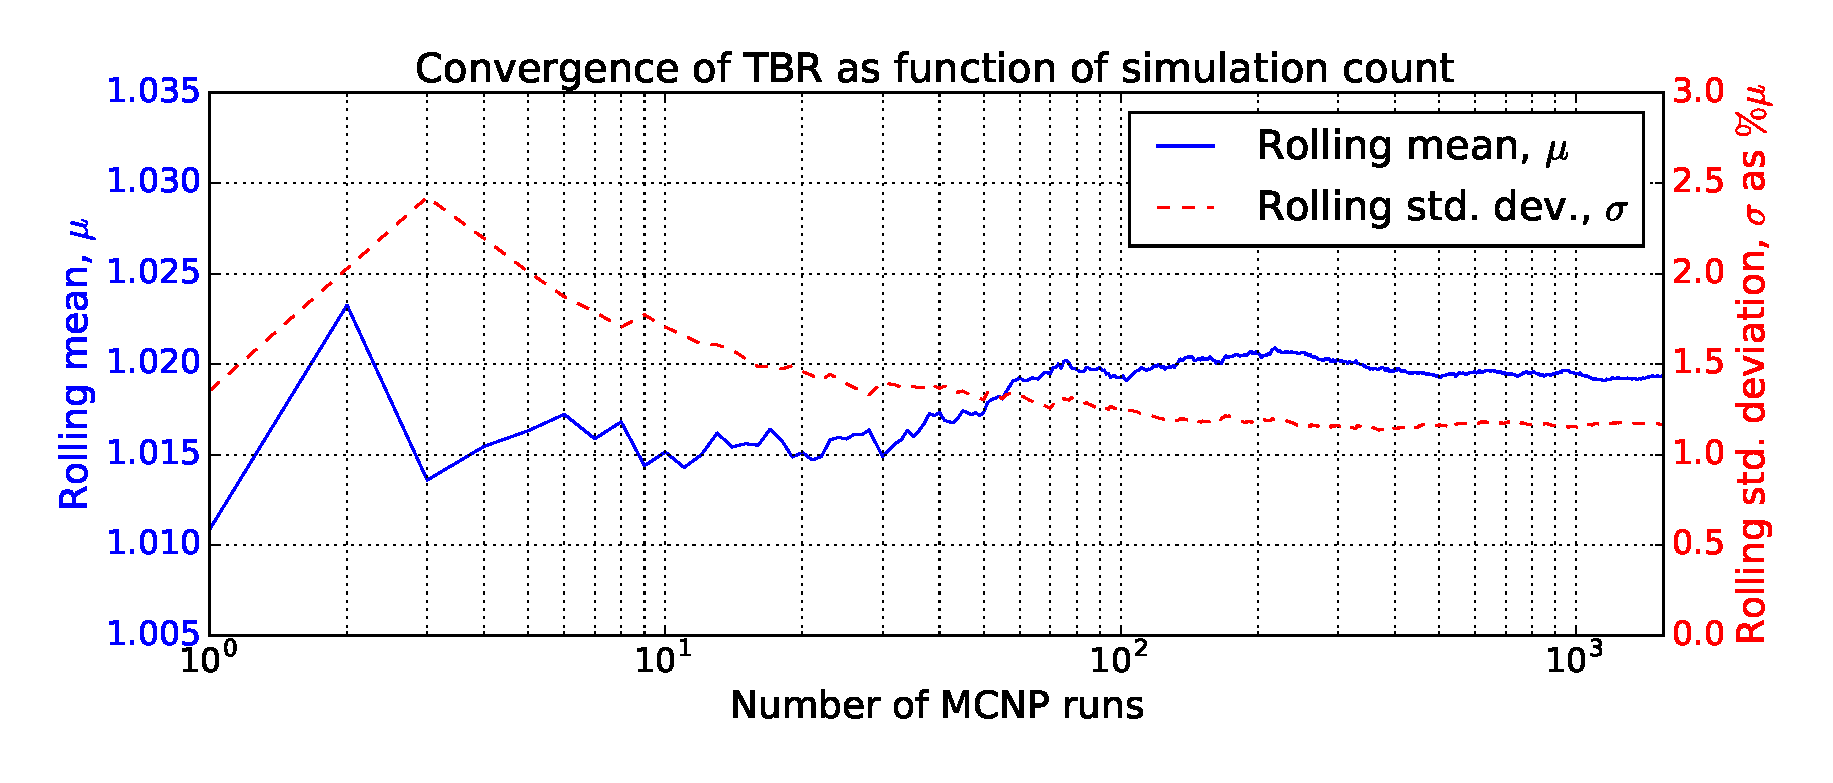
\includegraphics[width=\textwidth]{hcll_convergence_1559}
	\caption{The mean and standard deviation of the TBR distribution is presented as a function of the number of simulations. The TMC simulation can be seen to converge at approximately 400 MCNP runs. $\mu(400) \approx 1.02$ and $\sigma(400) \approx 1.14$.}
	\label{fig:convergence}
\end{figure}

The mean TBR value is 1.0193 whilst the median is 1.0200, with a one sigma standard deviation of 0.012 or 1.2\% of the mean. The TBR distribution is approximately normal, with a small skewness of -0.199, meaning the low-value TBR tail is longer than the high-value tail. Figure \ref{fig:tbr_n2n} shows the expected correlation between the n,2n cross-sections used in a given simulation and the TBR attained in that simulation.

\begin{figure}[ht]
%  \figuretitle{}
  \centering
	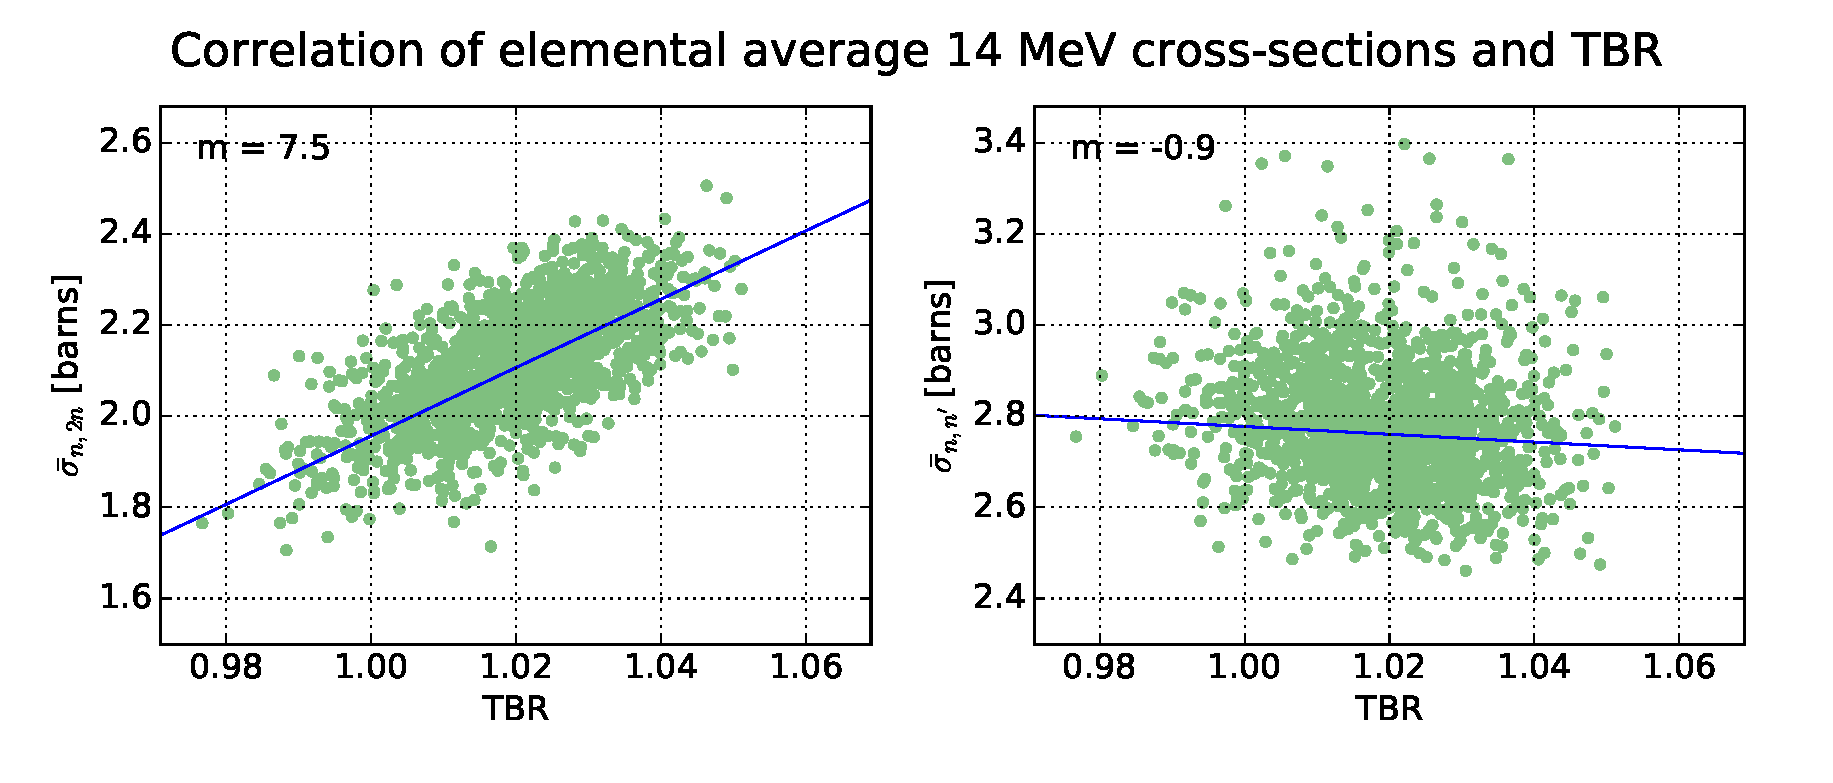
\includegraphics[width=\textwidth]{pb_tbr_n2n_el_corr}
	\caption{Above are scatter plots of average cross-sections for the n,2n (left) and elastic (right) channels against resulting TBR value. As the cross-sections for each of the three lead isotopes were varied in every simulation, so the cross-sections plotted here are the elemental average values denoted as $\overline{\sigma}_{n,2n}$ or $\overline{\sigma}_{n,n'}$, i.e. all three varied Pb isotopes contribute, weighted by their relative natural abundances. The n,2n cross-section is positively correlated with the TBR value as expected. There is less of a relationship between scattering and TBR.}
	\label{fig:tbr_n2n}
\end{figure}

%%%%%%%%%%%%%%%%%%%%%%%%%%%%%%%%%%%%%%%%%%%%%%%%%%%%%%%%%%%%%%%%%%%%%%%%%%%%%%%%%%%%%%%%%%%
% Let's compare the TBR with the parameter variations to see what it's most sensitive to! %
%%%%%%%%%%%%%%%%%%%%%%%%%%%%%%%%%%%%%%%%%%%%%%%%%%%%%%%%%%%%%%%%%%%%%%%%%%%%%%%%%%%%%%%%%%%

% Have TBR to job ID list (tbr_values files), but need something to couple job ID to xsdir and random file numbers
% Check Culham machines, /home/fthomas/projects/tmc/sims/13-...
% All optical model parameters mentioned in this Section can be adjusted, not only by means of a local §parameter file (see the optmodfileN keyword), but also via adjustable parameters through the v1adjust, v2adjust etc. keywords, with which the standard values can be multiplied. 

%%%%% WARNING ---->
% Even energy dependent adjustment of the geometry is possible as a last resort to fit data, using the rvadjustF, etc. keywords.
% Have we found a strong correlation between a fudge parameter and the TBR? Oh dear

Uncertainty propagation in Monte-Carlo type radiation transport problems has often previously been computed using linear perturbation theory approaches. Unfortunately these are only applicable for small changes in the input data. They are also unable to reproduce probability distributions of the integral quantity of interest \cite{Rising2012}. Whilst figure \ref{fig:tbr_distribution} shows a TBR distribution that is not tremendously skewed, that is not to say other fusion quantities will not be. Koning \& Rochman have demonstrated that fast and accelerator driven fission systems can have significantly skewed k$_{\mbox{eff}}$ values, best described by an Extreme Value Fit (EVD) \cite{Koning2008}.

\begin{figure}
%  \figuretitle{}
	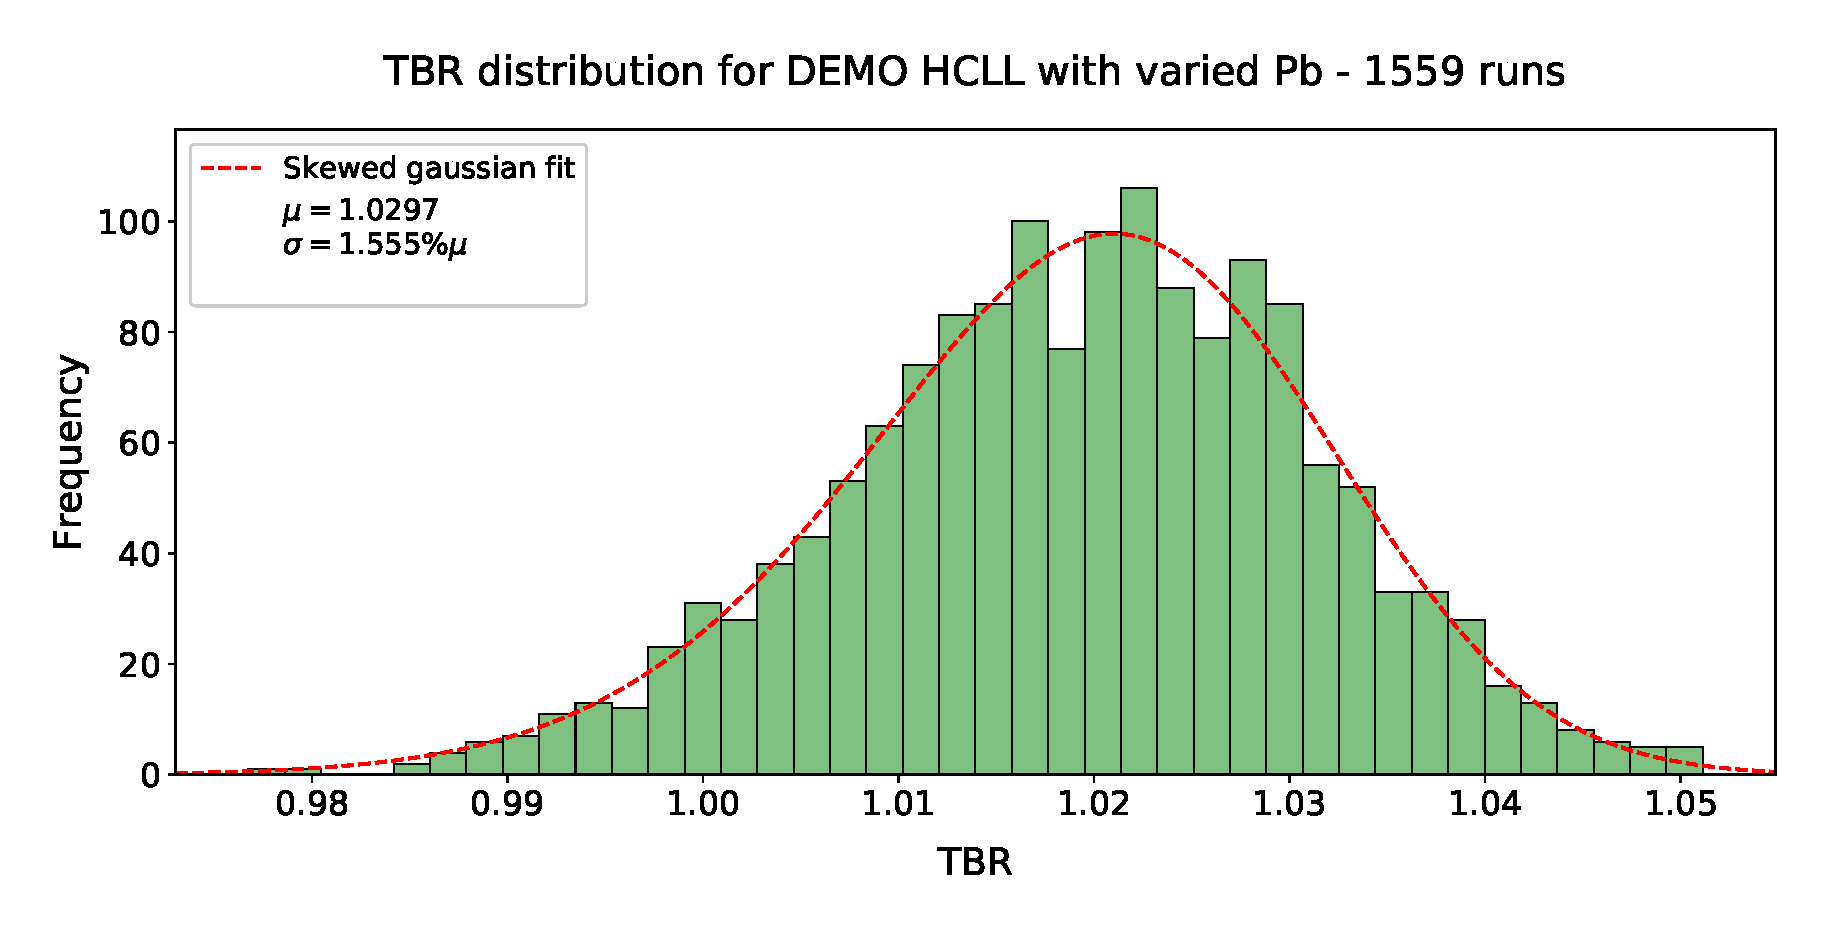
\includegraphics[width=\textwidth]{hcll_hist_1559}
	\caption{Histogram of TBR values computed with the TMC methodology.}
	\label{fig:tbr_distribution}
\end{figure}

\section{Conclusion}
TBR uncertainty has been computed with the TMC technique, investigating the contribution of uncertain nuclear data from the three major lead isotopes. The standard deviation is 1.2\% of the mean TBR. However, note that 5.8\% of the distribution is less than unity. While the average value may appear to be feasible, it should be stressed that there is a non-negligible probability of a value below a required limit. The TBR values are relatively low as this particular model has not been optimised for TBR and any practical design should have a TBR $\approx 1.1$ \cite{Fischer2015}, but in future design studies engineers should be aware of the probability of non-compliant operational parameters. 

The TENDL-2015 nuclear data investigated in section \ref{sec:data}, which is not necessarily Gaussian in shape, has yielded a TBR distribution with a small but finite negative skewness, an extended low-value tail. It is not possible to deduce this shape with more simplified approaches to uncertainty propagation such as linear perturbation theory.

Future work on TBR in HCLL could include the effect of other nuclides and elements which TBR is sensitive to including iron, as well as a completely correlated uncertainty propagation method employing lithium. 

More generally, when solving for integral quantities in nuclear fusion systems, thought should be given to fully-correlated uncertainty propagation and the form of the resulting probability distributions. In particular, whether a non-normal distribution with increased likelihood of extreme behaviour would have engineering design or safety implications for TBR, nuclear heating, fast flux, gas production or damage terms. Moreover, in all analyses for design applications the non-negligible probability of operational parameters in unacceptable regimes should be borne in mind.

